\documentclass[../main.tex]{subfiles}
\begin{document}
\chapter{Enrichissement des modèles qualitatifs : Modèle de logique linéaire temporel et méthode de sélection de communauté à façon \maxime{NE PAS LIRE}}
\label{enrichissement}
\minitoc
\newpage

%\doublespacing %% à utiliser pour faciliter la correction du manuscrit

\section{Introduction}
Ce chapitre \ref{enrichissement} symbolise le fruit terminal de cette thèse prenant en considération les limites et les avantages du modèle numérique du chapitre \ref{tango} et du modèle par raisonnement du chapitre \ref{ccmc}. Rappelons que l'objectif final est de trouver des pistes permettant d'analyser des communautés complexes tout en conservant, précision et explicabilité du résultat. Nous avons vu que le modèle discret (chapitre \ref{ccmc})  a permis l'étude de communautés complexes en redirigeant l'analyse sur les potentiels de coopération et de compétition de communautés bactériennes. Le point critique majeur de notre méthode est l'absence de fonction objective à optimiser, permettant d'affiner les résultats. Dans la littérature, il existe un outil, basé sur le même principe par raisonnement que nous, qui permet d'optimiser différentes fonctions objectives: taille de la communauté et nombre des échanges métaboliques \citep{Frioux2018}. Ces optimisations permettent de sélectionner des communautés candidates selon les deux critères précédents. Appliquer et étendre ces choix d'optimisation à notre modèle par raisonnement permettrait de (i) réduire les sorties d'un modèle par raisonnement, (ii) enrichir le modèle en apportant de la souplesse d'utilisation et (iii) laisser les utilisateurs et les utilisatrices définir les concepts de communautés à fort potentiel de coopération ou de compétition. Le second point de critique majeur de notre modèle discret est l'absence de la prise en compte de la temporalité. Au cours du chapitre \ref{tango}, nous avons vu que la concentration d'un métabolite au cours du temps n'évolue pas linéairement, mais passe par des phases qualitatives différentes: augmentation (forte ou faible), diminution (forte ou faible) ou encore, absence de changement. Par exemple, sur la Figure \ref{dfba_community} l'évolution discrète de la concentration de lactate est: forte augmentation, absence d'évolution puis diminution faible. De plus, lors de l'exploration du modèle de communauté, nous avons vu que le moment où un métabolite est consommé change l'hypothèse d'interaction. Par exemple, le lactose est d'abord consommé par \lactis puis par \freud, ne permettant pas de définir une hypothèse de compétition entre ces deux espèces. Enfin, nous avons montré la plus-value d'ajouter des contraintes biologiques sur la précision du modèle. Par exemple, le métabolisme des bactéries lactiques reste actif pendant la phase stationnaire permettant de produire de l'acide lactique et ainsi, expliquer les données biologiques. Dans la littérature, d'ajout de la temporalité dans un modèle par raisonnement il existe un formalisme logique introduit pas les travaux de Cabalar \citep{Cabalar2019} : la logique linéaire temporelle (LTL). Ce formalisme logique utilise le solveur \textit{telingo} qui combine l'ASP avec des contraintes temporelles. En associant ce formalisme avec le concept IA du raisonnement sur les actions et les changements (RAC), permettant de connaître la cause d'un changement d'un système, Cabalar permet d'expliquer à partir d'inférence de règles logiques temporelles, les observations. En revanche, il existe à notre connaissance, aucune application du un système biologique. En somme, une inférence de la temporalité et de contraintes biologiques dans le modèle de communauté aurait pour conséquence de réduire le nombre de solutions possibles en sélectionnant les modèles qui satisfassent ces contraintes et d'affiner les résultats du modèle logique existant. \\

Ainsi, nous verrons au cours de ce chapitre comment l'apport d'une souplesse et d'une facilité d'utilisation permet d'enrichir les possibilités de sélection d'une communauté candidate. Puis dans un second temps, nous verrons comment l'ajout de la temporalité en se basant sur le RAC permet d'apporter des connaissances temporelles supplémentaires par rapport au modèle dynamique du chapitre \ref{tango}. 


\section{Critères d'optimisation à partir de contraintes biologiques \textit{a priori}}
L'une des questions que nous nous sommes posés est la définition de la "meilleure" communauté pour répondre à un objectif. Les travaux de Frioux et ses collègues \citep{Frioux2018} propose de minimiser la taille de la communauté ainsi que les échanges métaboliques conduisant à la production de métabolites cibles. Or, au cours de discussions avec des biologistes, nous avons identifié que les choix de minimisation faits dans MISCOTO ne garantissaient pas l'obtention de la meilleure communauté. Cependant, enlever une optimisation ne permettrait pas de résoudre la combinatoire importante conduit par les interactions bactériennes. Une autre question sous-jacente est donc celle du choix de la fonction objective à optimiser. En complément de celles utilisées dans MISCOTO, nous avons calculés des potentiels de coopération et de compétition ainsi qu'étendu le vocabulaire existant avec les notions de substrats polyopsonistes et du nombre de contributeurs dans un échange. Ces options supplémentaires enrichissent le choix d'optimisation, contribuant à la définition d'une communauté à fort potentiel de coopération ou de compétition. Parmi l'ensemble de ces éléments (nombre d'échanges, substrats polyopsonistes etc.), il existe à notre connaissance, pas de consensus sur la description de la communauté avec de fortes propriétés coopératives/compétitives. Nous avons ainsi développé un prototype laissant l'utilisateur ou l'utilisatrice la possibilité de sélectionner des communautés selon un ensemble de contraintes pertinents pour leur domaine d'application. Ces contraintes se catégorisent en deux parties. La première consiste à filtrer la communauté selon la composition taxonomique de cette dernière. La seconde, consiste à optimiser des concepts du vocabulaire issu de la modélisation discrète des communautés sélectionnés préalablement. Afin de garantir une facilité d'utilisation, nous nous sommes basés sur le format YAML pour définir les contraintes. Dans la suite du chapitre nous allons vous présenter les nouvelles contraintes, comment le prototype s'articule et montrer sa souplesse et facilité d'utilisation.

\subsection{Méthodologie}
Lors du l'élaboration de ce prototype, nous avons consacré du temps à sa facilité d'utilisation. Nous allons donc vous présenter les contraintes supplémentaires, la base de fait créé à partir de ces contraintes et comment la ou le biologiste peut les utiliser. Dans un second temps, l'implémentation de ces nouvelles contraintes sous la représentation mathématique et sous le formalisme ASP.

\subsubsection*{Contraintes de sélection et interface utilisateur}
Puisque les contraintes de modélisation discrète ont été défini dans le chapitre \ref{ccmc}, nous allons uniquement décrire les nouvelles contraintes liées à la composition de la communauté.  Afin de faciliter la lisibilité et l'accessibilité, nous avons utilisés le YAML comme une interface claire servant de pont entre les biologistes et l'outil.

\paragraph*{Contrainte sur la taille des communautés.}
L'utilisateur ou l'utilisatrice peut choisir une sélection plus ou moins stringente des tailles de communautés qu'il ou elle souhaite. Ce prototype propose de filtrer les communautés en sélectionnant une taille fixe, c'est à dire, parmi l'ensemble des combinaisons possibles, seules les communautés qui ont exactement cette taille seront sélectionnées. Ou une taille bornée par des valeur minimales et maximales, seules les communautés dont leurs tailles sont comprises dans l'intervalle seront sélectionnées. 
%Un exemple de cette sélection est illustré par la Figure \ref{fig:selection-taille}. 

%\begin{figure}[h!]
%    \centering
%    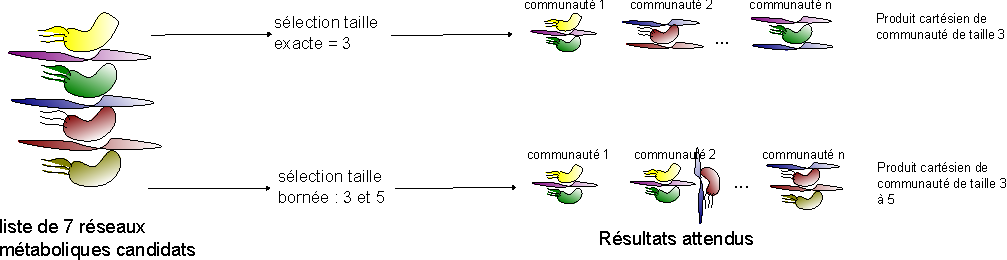
\includegraphics[scale=0.8]{img/enrichissement/figure_chapitre_renichissement.pdf} 
%    \caption{Exemple du principe de la sélection de communauté par sa taille.}
%    \label{fig:selection-taille}
%\end{figure}

Par exemple, un ou une biologiste aimerait obtenir l'ensemble des communautés qui ont une taille comprise entre \textbf{6} et \textbf{8}. Le fichier YAML d'entrée se structurerait ainsi:

\noindent
\begin{lstlisting}[style=yaml]
# Size constraints
SIZE:
  size: 
  lower bound: 6
  upper bound: 8
\end{lstlisting}

À partir de la lecture de ce fichier YAML, l'outil génère la liste de fait ASP, permettant de représenter les contraintes sous forme de connaissance:\\
\noindent
\begin{lstlisting}
lower_bound_size("6").
upper_bound_size("8").
\end{lstlisting}
 
Dans le cas où une taille fixe est demandée par les biologistes, seul le mot clé \texttt{size} est concerné. Par exemple, la demande "je ne veux que des communautés de taille \textbf{4}" se traduit par:
\begin{lstlisting}[style=yaml]
# Size constraints
SIZE:
  size: 4
  lower bound: 
  upper bound: 
\end{lstlisting}
Avec la \textbf{liste de faits ASP} suivante: \\
\begin{lstlisting}
lower_bound_size("4").
upper_bound_size("4").
\end{lstlisting}

Dans le cas où une taille fixe et une taille bornée sont renseignées, l'outil considère seulement la taille fixe.

\paragraph*{Contraintes sur la composition taxonomique bactérienne}
En plus de la taille, la ou le biologiste peut décider de la composition taxonomique, au grain de la souche, des communautés sélectionnées. Nous avons supposé que l'utilisateur ou l'utilisatrice connait un sous ensembles des souches bactériennes. Cette contrainte répond à des demandes biologiques telles que: "Au sein de ma communauté, je souhaite que les souches \textbf{XXX} et \textbf{YYL} soient présentes car elles permettent la libération de composés d'arômes d'intérêt, mais je ne veux surtout pas la souche \textbf{HHJ} et \textbf{KM} car elles sont en compétition avec les précédentes souches". Remarque, les raisons biologiques justifiants les intérêts pour ces souches ne sont pas prises en compte au sein de l'outil. Cette contrainte de présence absolue et d'interdiction se traduit respectivement dans le YAML part les clés d'entrée suivante: \texttt{always} et \texttt{forbid}:

\noindent
\begin{lstlisting}[style=yaml]
# Bacterial composition 
constraints
BACTERIAL COMPOSITION:
  always: 
    - XXX
    - YYL
  forbid: 
    - KM
    - HHJ
\end{lstlisting}

La liste de faits ASP à partir de ces contraintes sont les suivants:\\
\begin{lstlisting}
always("XXX").
always("YYL").
forbid("KM").
forbid("HHJ").
\end{lstlisting}


Nous avons également développé des contraintes supplémentaires sur la composition taxonomique de la communauté: associations interdites et obligatoires, nommées respectivement \texttt{forbidden asso} et \texttt{mandatory asso}. Une demande biologique illustrant ces propos serait: "S’il existe une communauté où une des souches \textbf{XV}, \textbf{FV} ou \textbf{JH} est présente, alors l'ensemble de ces souches doit être présent également. En revanche, tant que l'ensemble des souches \textbf{FV}, \textbf{PP} et \textbf{FT} n'est pas présent \underline{ensemble} dans la même communauté, mais que des sous-ensembles le sont, je considère la communauté valide." Ces contraintes diffèrent de \texttt{always} et de \texttt{forbid} du fait des notions d'ensemble, et l'ensemble nul est considéré comme valide du point de vue méthodologie: par exemple,  une communauté où ni \textbf{XV}, \textbf{FV} ou ni \textbf{JH} n'est présente, est valide. Ces associations permettent également de définir des différents groupes de souches interdites ou obligatoires. Par exemple, en complétant la demande: "En plus de ces associations, si une des souches \textbf{AA} et \textbf{ZS} est présente alors l'ensemble doit être présent également. Cependant, l'ensemble \textbf{PO} et \textbf{ML} ne doit pas être ensemble". Grâce au YAML, ces contraintes sont formalisables comme suit:


\noindent
\begin{lstlisting}[style=yaml]
# Bacterial composition 
constraints
BACTERIAL COMPOSITION:
forbidden asso: 
    - 
      - FV
      - PP
      - FT
    - 
      - PO
      - ML

  mandatory asso: 
    - 
      - XV
      - FV
      - JH
    - 
      - AA
      - ZS
\end{lstlisting}
Les différents groupes d'ensemble interdits (resp. obligatoires) sont symbolisé par \texttt{\_} de la ligne 5 et 9 (ligne 14 et 18). Ces groupes sont également visibles dans liste de faits ASP générée à partir de ces contraintes et se traduisent par le numéro en amont de la souche et sont définis automatiquement à la lecture du fichier YAML:\\

\noindent
\begin{minipage}[t]{0.45\textwidth}
\begin{lstlisting}
forbidden_asso("0","FV").
forbidden_asso("0","PP").
forbidden_asso("0","FT").
forbidden_asso("1","PO").
forbidden_asso("1","ML").
\end{lstlisting}
\end{minipage}% % leave no gap
\hspace{2em}\begin{minipage}[t]{0.5\textwidth}
\begin{lstlisting}
mandatory_asso("0","XV").
mandatory_asso("0","FV").
mandatory_asso("0","JH").
mandatory_asso("1","AA").
mandatory_asso("1","ZS").
\end{lstlisting}
\end{minipage}

\paragraph*{Flexibilité des fonctions objectives.}
Laisser le choix à l'utilisateur ou l'utilisatrice d'optimiser une ou plusieurs fonctions objectives correspond à l'enrichissement majeur du modèle logique. Comme nous avons vu précédemment, le choix de la fonction objective est important et sa modularité auprès de l'utilisateur ou l'utilisatrice l'est tout autant. Notre prototype d'outil prend actuellement les choix d'optimisation suivant: maximiser ou minimiser les échanges métaboliques, les métabolites cibles à produire, le scope métabolique et le nombre de substrats polyopsonistes. À partir du fichier d'initialisation YAML, les contraintes de maximisation ou de minimisation sont directement écrits ainsi:

\noindent
\begin{lstlisting}[style=yaml]
# Optimisation
OPTIMISATION: 
  - max
  - max

# Objectif
OBJ:
  - target
  - exchanged
\end{lstlisting}

Les lignes 3 et 4 indiquent le choix de l'optimisation que l'utilisateur ou l'utilisatrice souhaite faire, et les lignes 8 et 9 sont les objectifs possibles décrits plus haut. Dans cet exemple, le ou la biologiste veut en \underline{premier} maximiser la production d'un ensemble de cibles, puis, dans un \underline{second temps}, maximiser les métabolites échangeables. L'implémentation de cette contrainte se traduit de la façon suivante en ASP:\\

\begin{lstlisting}[label=lst:optimisation]
#maximize {1@1,M:target(M), pscope(M,_,_) }; 0@1}.
#maximize {1@2,S:exchanged(S); 0@2}.
\end{lstlisting}

Les priorités d'optimisation sont traduites par \texttt{1@1} et \texttt{1@2}, dans lequel la ligne 1 maximise le nombre de métabolites cibles présents dans le scope communautaire. \maxime{Adapter selon le nouveau formalisme développé dans CCMC ? ou mettre des noms plus communs pour aider la compréhension ?} 

\subsubsection*{Implémentation des nouvelles contraintes}
Nous venons de voir comment nous avons construit notre base de faits utiles pour formaliser les règles et les contraintes, conduisant à la sélection des communautés. Dans la suite de ce chapitre, nous allons formaliser les différentes règles et contraintes en ASP et expliciter formalisme mathématique. 

\paragraph*{Sélection par la taille de communauté}
Au sein du programme ASP, nous avons sélectionner les communautés par taille de la façon suivante:
\begin{lstlisting} [label=lst:taille]
lower_bound_size {chosen_bacteria(X):bacteria(X)} upper_bound_size.
\end{lstlisting}

Le listing \ref{lst:taille} sélectionne un sous ensemble de taille minimal \texttt{lower\_bound\_size.} et de taille maximal \texttt{upper\_bound\_size.} parmi l'ensemble \texttt{chosen\_bacteria(X)}, où X est dans le domaine défini par l'ensemble des bactéries (\texttt{bacteria}). Cela revient à sélectionner au hasard des bactéries (\texttt{chosen\_bacteria(X)}) parmi l'ensemble des bactéries initialement défini \texttt{bacteria}, où le nombre de bactéries sélectionner ne peut-être plus grand que \texttt{upper\_bound\_size.} et plus petit que \texttt{lower\_bound\_size.}\\

Mathématique, soit $t$ un sous-ensemble de taxon appartenant à l'ensemble de taxon \Ts, où un taxon correspond à une bactérie, la cardinalité $\vert t \vert $ doit être compris entre les valeurs $min$ et $max$:

\[
\forall t \in \Ts 
\]
\[
min<\vert t \vert <max
\]

\paragraph*{Sélection par la composition taxonomique au grain de la souche.}
Nous avons laissé la possibilité à l'utilisateur et à l'utilisatrice de filtrer sur la composition taxonomique de la communauté, avec les prédicats \texttt{always},\texttt{forbid},\texttt{mandatory\_asso} et \texttt{forbidden\_asso}.  

Le prédicat \texttt{always}, représentant un taxon qui doit être présent dans toutes les communautés possibles est implémenté en ASP comme suit:

\begin{lstlisting} [label=lst:always]
:- always(X); not chosen_bacteria(X).
\end{lstlisting}

Cette règle ne dispose pas de tête, on parle alors de contrainte d'intégrité. Elle se lit comme suit: parmi l'ensemble de bactérie initial, nous ne voulons pas les communautés où la bactérie définit par le prédicat \texttt{always(X)} n'est pas présente. La double négation étant lourde, nous pouvons traduire ainsi: sélectionne l'ensemble des communautés où la bactérie présumé \texttt{always} est présente. 

Mathématiquement, soit $A$ l'ensemble de bactéries obligatoirement présent dans la communauté:
\[
\forall t \in \Ts \text{ si } \forall A \in t 
\]

Concernant les bactéries qui ne doivent pas être présent dans la communauté, le code ASP ainsi que le formalisme mathématique est très ressemblant:

\begin{lstlisting} [label=lst:forbid]
:- chosen_bacteria(X); forbid(X) : chosen_bacteria(X).
\end{lstlisting}

Cela se traduit par: les communautés qui possèdent un ensemble de bactéries interdites (\texttt{forbid(X)}) parmi l'ensemble des bactéries tirées au sort ne doivent pas être sélectionnées. Mathématiquement, on appelle l'ensemble de bactérie interdit $F$, et est défini comme suit:

\[
\forall t \in \Ts \text{ si } \forall F \not \in t 
\]

Nous avons également défini des associations obligatoires (\texttt{mandatory\_asso}) et interdites (\texttt{forbidden\_asso}). Pour rappel, l'utilisateur ou l'utilisatrice pouvait définir des groupes d'association, nommé \texttt{group\_forbidden(G)} dans le cas des associations interdites. Ce prédicat regroupe l'ensemble des groupes (\texttt{G}) que la ou le biologiste a défini dans le fichier de configuration YAML. Nous avons défini les associations obligatoires en 3 parties.

Dans le listing \ref{mandatory1}, les communautés sélectionnées (\texttt{selected\_bacteria(X)}) ont obligatoirement toutes les bactéries de l'ensemble des associations obligatoires parmi l'ensemble de bactéries préalablement choisis (\texttt{chosen\_bacteria(X1) : mandatory\_asso(\_,X1).}).

\begin{lstlisting} [label=mandatory1,caption=Règle numéro 1 pour définir les associations obligatoires, captionpos=b]
selected_bacteria(X) :- chosen_bacteria(X); 
		  chosen_bacteria(X1) : mandatory_asso(_,X1).
\end{lstlisting}

Il faut ensuite rajouter les communautés où aucune des bactéries des associations obligatoires n'est présent parmi l'ensemble de bactéries préalablement défini (\texttt{not chosen\_bacteria(X1) : mandatory\_asso(\_,X1).}). Ce calcul est illustré par le code dans le llisting \ref{mandatory2}

\begin{lstlisting} [label=mandatory2,caption=Règle numéro 2 pour définir les associations obligatoires, captionpos=b]
selected_bacteria(X) :- chosen_bacteria(X);
	    not chosen_bacteria(X1) : mandatory_asso(_,X1).
\end{lstlisting}

Enfin, pour une question de visualisation des solutions, nous avons ajouté la contrainte d'intégrité \ref{mandatory3} qui ne montre que les communautés filtrées par les associations obligatoires.

\begin{lstlisting} [label=mandatory3,caption=Règle numéro 3 pour définir les associations obligatoires, captionpos=b]
:- chosen_bacteria(X); not selected_bacteria(X).
\end{lstlisting}

Mathématiquement, soit $O$ l'ensemble des bactéries des associations obligatoires, et $o_i \forall i \in O$. Les associations obligatoires sont définies comme:

\[
\forall O \in \Ts \text{ si } o_i = t \text{ alors } \forall o_i \in t 
\]

Enfin, pour définir les associations interdites au sein d'une communauté (voir listing \ref{lst:forbidden}, les communautés sélectionnées ne doivent pas posséder l'ensemble des bactéries interdites parmi les communautés déjà sélectionnées (\texttt{chosen\_bacteria(X2) : forbidden\_asso(G,X2).})

\begin{lstlisting} [label=lst:forbidden, caption=Règle définissant les associations interdites, captionpos=b]
:- chosen_bacteria(X); group_forbidden(G);
		chosen_bacteria(X2) : forbidden_asso(G,X2).
\end{lstlisting}

Mathématiquement, soit $I$ l'ensemble des bactéries des associations interdites et $I_i \forall i \in I$. Les associations interdites sont alors définies comme:

\[
\forall I \in \Ts \text{ si } \forall I_i \not \in t \text{ alors } I_i \in t 
\]

\begin{figure}[h!]
    \centering
    \includegraphics{example-image-a}
    \caption{Montrer en image le workflow complet en illustration. Montrer la facilité d'utilisation pour les biologistes et les liens entre chaque modification faite par l'utilisateur et la contrainte formalisés.}
    \label{fig:my_label}
\end{figure}
\newpage

\subsection{Résultats préliminaires}
Nous venons de décrire et détailler la base de connaissance nécessaire pour sélectionner des communautés à façon. Dans cette sous-section, nous allons dans un premier temps identifier des questions biologiques provenant d'un retour d'expérience sur les précédents chapitres ainsi que de discussions avec les biologistes, et comment l'outil de sélection permet d'y répondre. Puis dans un second temps, nous allons appliquer notre méthode de sélection de communauté à façon sur le jeu de données du papier M2M \citep{Belcour.2020} afin de montrer son efficacité à passer à l'échelle.

\subsubsection*{Exemples}
Toutes les questions ci-dessous vont chercher à identifier des ensembles de communautés candidates pour des objectifs métaboliques supposés connus. Les questions seront présentées des plus larges au plus précises. Nous utiliserons les réseaux métaboliques reconstruits à l'échelle du génome de Weiss \citep{Weiss2022}. Ils ont été reconstruits avec l'outil GapSeq\citep{Zimmermann2021} et un consortium bactérien permettant une analyse des interactions métabolique de l'intestin de souris a été créé.


\paragraph*{\textit{Pour une communauté de taille 5, existe-t-il une communauté qui métaboliste l'ensemble des acides aminés?}}
Cette question nous permet d'identifier les deux contraintes à utiliser au sein de l'outil: la liste des composés que l'on doit produire, \textit{i.e.} les acides aminés (AA), ainsi que la taille de la communauté finale, \textit{i.e.} 5. 

Le fichier initial est donc constitué des informations suivantes:
\begin{lstlisting}[style=yaml]
# Size constraints
SIZE:
  size: 5
\end{lstlisting}

N'ayant précisé aucune optimisation, l'ensemble des cibles, que sont les acides aminés, devront être dans le scope de la communauté. Le résultat pour cette situation est \textbf{unsatisfiable}. Cela signifie qu’il n’existe pas de modèles permettant de satisfaire les contraintes de l'utilisateur ou de l'utilisatrice, et donc aucune communauté de taille n'a été trouvé comme étant capable de métaboliser l'ensemble des acides aminés.
Le premier réflexe de l'utilisateur ou de l'utilisatrice est de formuler la demande de façon à relâcher les contraintes. La contrainte la plus forte ici consiste à obtenir au moins une communauté permettant de l'ensemble des \textbf{métaboliser les acides aminés}. Une reformulation possible serait: métaboliser un \textbf{maximum} d'acide aminé. En appliquant cette modification nous obtenons une communauté composée des souches \textit{I48}, \textit{KB1m}, \textit{YL44}, \textit{YL45}, \textit{YL27}.\\

\paragraph*{\textit{Pour une communauté composée de 6 taxa, laquelle permet la plus grande production métabolique sans les échanges métaboliques?}} 
Nous avons 2 types de contraintes: 2 optimisations, que sont la maximisation du scope communautaire et la minimisation des échanges métaboliques, et taille, et se traduit comme suit dans le fichier d'initialisation:

\begin{lstlisting}[style=yaml]
# Size constraints
SIZE:
  size: 5
  
  # Optimisation
OPTIMISATION: 
  - max
  - min

# Objectif
OBJ:
  - scope
  - exchanged
\end{lstlisting}

La meilleure communauté, selon le solveur, possède 797 échanges et 1010 métabolites sont productibles en communauté. En plus de connaître la meilleur composition taxonomique répondant à ces contraintes, le vocabulaire contrôlé développé dans le chapitre \ref{ccmc} est également accessible: les métabolites échangeables, les consommateurs et producteurs intervenant dans l'échange, les substrats polyopsonistes, les potentiels de coopération et de compétition.



\paragraph*{\textit{A partir d'une communauté de 150 réseaux métaboliques de l'intestin, j'aimerai une étudier une communauté de composé de 6 à 8 taxons garantissant une productibilité d'un maximum des 23 composés d'intérêts}}
En plus de ces contraintes, il y a des contraintes de composition taxonomique que sont: \textit{les réseaux métaboliques GCA\_003433685, GCA\_003433675 et GCA\_003433665 doivent-être \underline{présent}, GCA\_003433745, GCA\_003433755 et GCA\_003433765 doivent \underline{jamais apparaître} dans la ou les communautés. Les ensembles GCA\_003433795, GCA\_003433825 et GCA\_003433845 \underline{ou} GCA\_003433855 et GCA\_003433865 ne doivent pas être présents. En revanche, les ensembles GCA\_003433905, GCA\_003433925 et GCA\_003433945 \underline{ou} GCA\_003433955 et GCA\_003433985 doivent être présent.} Cette demande factice test le passage à l'échelle de la méthode. Nous avons donc utilisé 150 réseaux métaboliques reconstruits dans le chapitre \ref{ccmc} :\\

\noindent
\begin{minipage}[t]{0.4\textwidth}
\textbf{contrainte d'entrée}: 
\begin{lstlisting}[style=yaml]
# Size constraints
SIZE:
  size: 
  lower bound: 6
  upper bound: 8

# Bacterial composition
 constraints
BACTERIAL COMPOSITION:
  in: 
    - GCA_003433685
    - GCA_003433675
    - GCA_003433665
  out: 
    - GCA_003433745
    - GCA_003433755
    - GCA_003433765
  forbidden asso: 
    - 
      - GCA_003433795
      - GCA_003433825
      - GCA_003433845
    - 
      - GCA_003433855
      - GCA_003433865

  mandatory asso: 
    - 
      - GCA_003433905
      - GCA_003433925
      - GCA_003433945
    - 
      - GCA_003433955
      - GCA_003433985
      
# Optimisation
OPTIMISATION: 
  - max

# Objectif
OBJ:
  - target
\end{lstlisting}
\end{minipage}% % leave no gap
\hspace{2.5em}\begin{minipage}[t]{0.5\textwidth}
\textbf{sortie}: 

\begin{lstlisting}
Answer: 1

GCA_003433925.
GCA_003433985.
GCA_003433685.
GCA_003433675.
GCA_00343390.
GCA_003433945.
GCA_003433665.
GCA_003433955.
\end{lstlisting}
\textbf{Performance}: 

Models: 1

Time: 197.120s 

CPU Time: 196.781s\\

En maximisant une liste de composés d'intérêt (23) et à partir des paramètres ci-dessus, nous avons trouvé une communauté candidate en environ 3 minutes et 30 secondes.
\end{minipage}

\section{Discussion et conclusion}
Cette première exploration d'enrichissement d'un modèle logique a répondu aux remarques majeures que nous avons énoncées plus haut: filtrer le nombre de solutions d'un modèle logique et optimisation de fonctions objectives. En effet, l'outil développé dans le chapitre \ref{ccmc} permet de donner une indication des potentiels de coopération et de compétition de communautés microbiennes mais ne permet pas d'identifier les critères permettant de l'affirmer. Avec ce prototype, nous avons proposé un moyen de sélectionner la meilleure communauté selon les critères de l'utilisateur ou de l'utilisatrice, et par extension, de définir la communauté avec un fort potentiel de coopération ou de compétition. Cela a été possible en ajoutant une optimisation d'une ou de plusieurs fonctions objectives. La plus-value par rapport au logiciel MISCOTO est que l'utilisateur ou l'utilisatrice choisi la fonction objective qu'il ou elle souhaite optimiser.\\

Cependant, aucune validation expérimentale n'a été faite à ce jour. Au regard de la littérature concernant la création de communauté à façon, une validation expérimentale est nécessaire pour créer une bonne communauté synthétique \citep{Sharma2020,Vazquez-Castellanos2019}. Par exemple, Macchi et ses collègues \citep{Macchi2021} ont construit une communauté bactérienne à partir de 6 génomes isolés pour la dégradation du phénanthrène. \\

Vis à vis des interactions bactériennes, ce prototype permet de se concentrer essentiellement sur le potentiel de coopération d'une communauté bactérienne. Concernant le potentiel de compétition uniquement défini par les substrats polyopsonistes, c'est à dire un nutriment qui est co-consommé, l'ajouté de la temporalité semble être un bon moyen pour améliorer la prédiction de la compétition. En effet, dans le chapitre \ref{tango}, le lactose est bien co-consommé mais pas au même moment dans le temps, empêchant de définir un lien de compétition pour ce substrat. Afin d'essayer de prendre en compte une pseudo-temporalité au sein des modèles logiques, nous allons utiliser la logique temporelle de Cabalar \citep{Cabalar2019}.


\newpage

\section{Intégration d'une temporalité réactionnelle}
La logique linéaire temporelle (LTL), à notre connaissance, n'a jamais été appliquée dans un contexte biologique. Pourtant, dans son domaine d'application IA, l'inférence de règles temporelles permet d'affiner les prédictions en proposant des explications séquentielles. Brièvement, Cabalar se base sur le problème de raisonnement sur les actions et le changement (RAC). Il en existe 5: (i) la \textbf{simulation}; étant donné un état initial du système et une suite d'actions, la simulation permet de prédire l'état du système à un temps futur. (ii) L'\textbf{explication}; étant donné un état initial et un état futur du système, l'explication propose une séquence d'état intermédiaires du système menant de l'état initial à l'état final. (iii) \textbf{Planification}; étant donné un état initial du système et un objectif, la planification propose une séquence d'actions, éventuellement non-déterministes, garantissant l'objectif. (iv) \textbf{Diagnostique}; à partir d'une définition de transitions d'état normal et anormal ainsi qu'un ensemble d'états observés (normal et anormal),  le diagnostique propose un ensemble minimal de transitions expliquant les observations anormales. (v) \textbf{Vérification}, validation d'une propriété temporelle du système (comme sûreté, vivacité ou équité) ou une propriété de représentations (comme l'équivalence de modèles). \\

Le premier défi est l'application de ces concepts RAC à la biologie des systèmes. Nous avons donc associé le système à une communauté de GEMs et les actions à des activations de réactions. Ainsi, chaque nouvelle activation d'une réaction, selon l'algorithme d'expansion du réseaux métabolique d'Ebenhöh, consistera un nouvel état du système. En prenant un exemple simple de la communauté fromagère du chapitre \ref{tango}, nous savons que le propionate est produit à partir du lactate. Remarquons ici que nous ne précisons pas les organismes pour le moment. À partir de cette information nous pouvons déduire \textit{a minima} une relation de dépendance logique temporelle, qui est: pour qu'\textit{a un moment de la cinétique de fermentation} le propionate soit productible, il faut que le lactate soit productible \textit{avant}. En appliquant la LTL à des réseaux métaboliques, les notions temporelles \textit{un moment} et \textit{avant} seront définies selon la longueur du chemin menant à la production du composé: propionate. Au sein de la LTL, le solveur,  \textit{telingo}, cherche à minimiser la taille du chemin. Ainsi, à partir d'un ensemble de nutriments disponibles dans le milieu extracellulaire, un ensemble fini de voies métaboliques mène à la production d'un composé cible, et \textit{ \textit{ \textit{telingo}}} priorise le chemin le plus court, c'est à dire le nombre réaction le plus faible. De ce fait, la temporalité n'est pas représentée comme une dimension, tel que présent dans le dFBA par exemple, mais par une séquence d'actions, activation ou non d'une réaction: on parle de \textit{temporalité réactionnelle}. Dans la suite de ce chapitre nous allons définir les cas d'utilisation de Cabalar et les appliquer à la communauté du chapitre \ref{tango}.


\subsubsection*{Inférence temporelle dans la programmation logique}

\paragraph*{Solveur \textit{ \textit{ \textit{telingo}}}}
Nous avons vu que les modèles numériques, contrairement aux modèles logiques, pouvaient intégrer une dimension temporelle et ainsi analyser d'autres propriétés du système biologique. Il existe un formalisme informatique, nommé \textit{logique temporelle linéaire} ou LTL, qui permet d'introduire une notion de temporalité au sein des modèles logiques. 

Ce modèle de logique par raisonnement se base sur le même formalisme que celui décrit dans le chapitre \ref{ccmc}: une base de faits, des règles et contraintes doivent-être générées. \textit{telingo}permet d'intégrer des contraintes temporelles et les règles et contraintes utilise les opérateurs logiques temporels décrits dans la Figure \ref{fig:syntaxe}.

 \begin{figure}[h!]
	\centering
    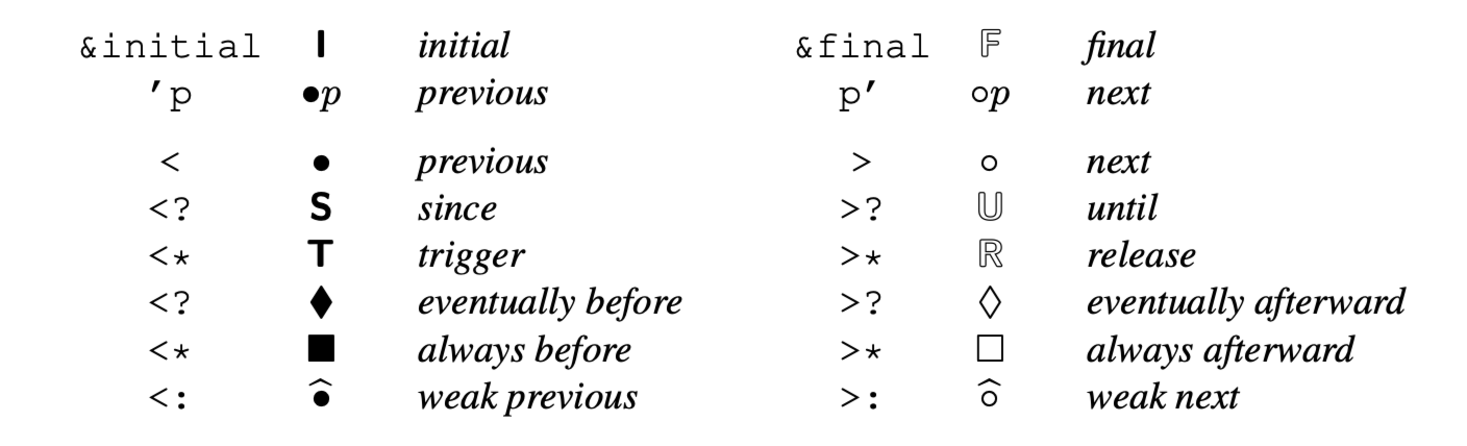
\includegraphics[width=\textwidth]{img/enrichissement/syntaxe_telingo}
    \caption{Opérateurs temporels du futur et du passé en \textit{telingo}et logique temporelle issue de \citep{Cabalar2019}}
    \label{fig:syntaxe}
\end{figure}

Dans l'exemple ci-dessous, nous avons défini une proposition vraie tout le temps : Quelque chose est \textit{chargé} si \textbf{au temps précédent} il a été \textit{chargé} et qu'il n'est pas \textit{déchargé}.  

\begin{lstlisting}[mathescape=True]
    charge :- $\square$ ($\bullet$ charge; not decharge)
\end{lstlisting}

À partir de cette nouvelle synthaxe, nous avons créé une communauté jouet du chapitre \ref{tango} afin d'appliquer la LTL et d'illustrer la temporalité réactionnelle au moyen de 3 concepts RAC: \textbf{planification}, \textbf{vérification} et \textbf{explication}. 

\subsection{Démarche à suivre}
Ce formalisme logique est une extension du formalisme décrit dans le chapitre \ref{ccmc} mais n'ayant jamais été appliqué sur des réseaux métaboliques, nous avons représenté les réseaux métaboliques de \freud, \plantarum et \lactis de manière simplifiée et minimaliste. Ce choix méthodologique a été imposé pour deux raisons: éviter dans un premier temps la problématique du passage à l'échelle et dans un second temps, permettre de résoudre les défis rencontrés lors de l'application des concepts de Cabalar. Dans les sous-sections qui suivent, nous présenterons les différents cas d'utilisation de Cabalar ainsi que leur résolution à partir d'une communauté factice, puis, l'application de ces concepts sur les réseaux métaboliques du chapitre \ref{tango}.

\subsection{Explication des concepts de Cabalar}

\subsubsection*{Ensemble de règles en \textit{telingo}pour la modélisation d'une communauté de bactéries}

\paragraph*{Scope}
Nous avons redéfini le vocabulaire exprimé dans le chapitre \ref{ccmc} en intégrant le vocabulaire temporel de la LTL. Ainsi, les notions de réactions activées et de composés productibles deviennent:

\begin{lstlisting}[label = lst:isActivated, caption = Règle d'activation d'une réaction, captionpos=b ]
0{isActivated(Rea,Org)}1 :- product(Compound,Rea,Org,_) ;
'producible(Reactant,Org) : reactant(Reactant,Rea,Org,_).
\end{lstlisting}

\begin{lstlisting}[label=lst:productible, caption = Règle de productibilité d'un composé, captionpos=b]
producible(Compound,Org):-  product(Compound,Rea,Org,_),
isActivated(Rea,Org).
\end{lstlisting}

Les contraintes exprimées dans les listings \ref{lst:isActivated} et \ref{lst:producible} signifient qu'une réaction est activée si l'ensemble des réactants ont été produits \textit{avant} (représenté par l'apostrophe \texttt{'}). Un composé est considéré comme productible si c'est un produit d'une réaction et qu'elle est activée.

L'évolution de la concentration d'un métabolite au cours du temps n'étant pas inférée dans le modèle, nous ne pouvons déterminer quand une réaction n'est plus activée. Nous assumons alors que si une réaction est activée une fois elle ne peut l'être une seconde fois. Cette règle s'exprime sous la proposition logique suivante :

\begin{lstlisting}[label=lst:notactivated, caption = Règle interdisant qu'une réaction soit activée deux fois, captionpos=b]
not isActivated(Rea,Org) :- not not &tel{ <? isActivated(Rea,Org)},
 reaction(Rea,Org).
\end{lstlisting}

% En revanche, déterminer quand est-ce qu'un métabolite devient polyopsoniste est possible. Ainsi, en utilisant le formalisme logique, une réaction n'est pas activée si celle-ci a déjà été activée dans le passé.

\paragraph*{Disponibilité des nutriments nouvellement productibles}
Avec cette notion temporelle à l'échelle d'une réaction, un composé produit en amont doit-être disponible pour une réaction qui se situerait en aval. La Figure \ref{disponible} illustre ce concept que nous avons développé. A partir du composé extracellulaire \texttt{Ae}, le composé C est productible au temps réactionnel 2. Il est ainsi disponible pour la réaction situé 2 temps réactionnel en aval, la réaction R4. 

    \begin{figure}[H]
        \begin{center}
            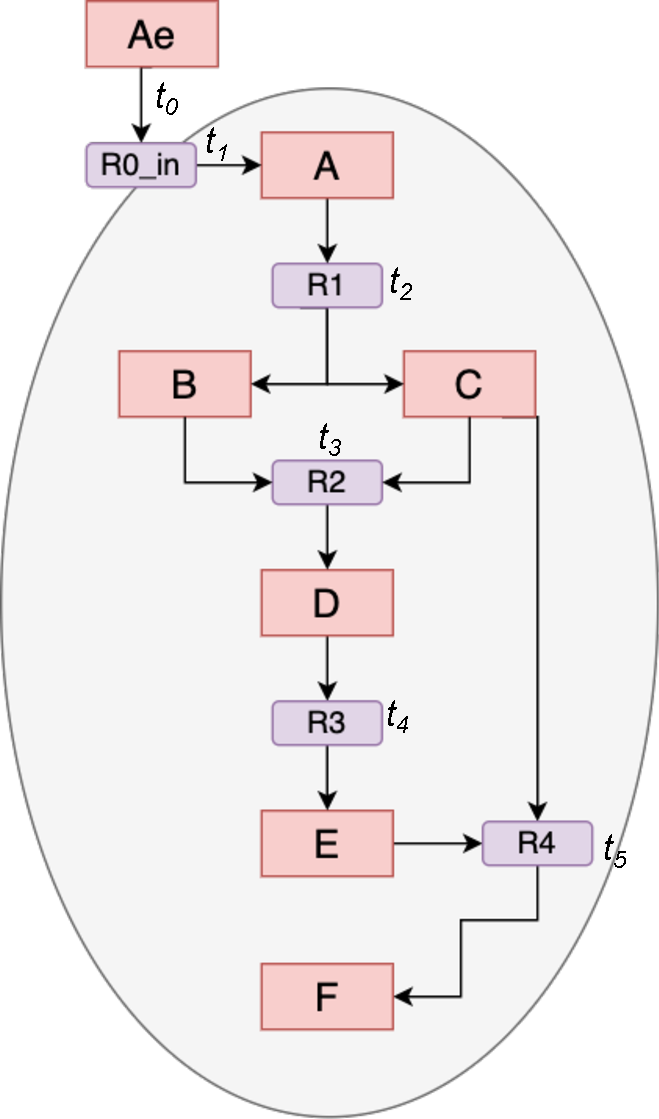
\includegraphics[scale=0.50]{img/enrichissement/reutilisation.pdf}
                \caption{Réutilisation du composé C par la réaction R4 où C était productible 2 étapes avant }
            \label{disponible}
        \end{center}
    \end{figure}
    
Avec cette nouvelle propriété, la définition de réaction activée est redéfinie ainsi: Une réaction est activée si tous les réactants de la réaction ont été productible avant (représenté par l'apostrophe à ligne 2):

\begin{lstlisting}
disponible(Compound,Org) :- producible(Compound,Org).
disponible(Compound,Org) :- 'disponible(Compound,Org).
\end{lstlisting} 

Bien entendu, au sein d'une communauté bactérienne, nous observons des échanges métaboliques. Les métabolites échangés ont été considérés comme productibles ils deviennent alors disponibles pour l'ensemble des membres de la communauté.

\subsection{Application de \textit{telingo} sur des organismes jouets}
Nous venons de voir les règles essentielles permettant de modéliser une communauté bactérienne avec la synthaxe temporelle. Dans les sections suivantes nous verrons l'applications du formalisme \textit{telingo} sur le des communautés jouets afin de vérifier si les concepts RAC s'adaptent bien sûr à la biologie des systèmes. Les règles et les contraintes utilisées pour modéliser les concepts RAC ne seront pas expliquées, seul l'aspect temporel sera mis en avant.

\subsubsection*{Planification}
Nous avons dès à présent les éléments nécessaires pour modéliser les cas d'application de Cabalar. Pour cela nous avons utilisé les réseaux métaboliques illustré par les Figures \ref{fig:planification} et \ref{fig:explication}. Dans le cas de la planification, l'objectif à atteindre était de déterminer la communauté minimale pour la production du composé Ne. Dans la figure \ref{fig:planification}, ce composé peut être produit soit par l'organisme 1 seulement et par l'organisme 2 par l'intermédiaire de 2 échanges métaboliques. La sortie du modèle est indiquée par le chemin en vert validant ainsi la prédiction.

\begin{figure}[H]
    \begin{center}
        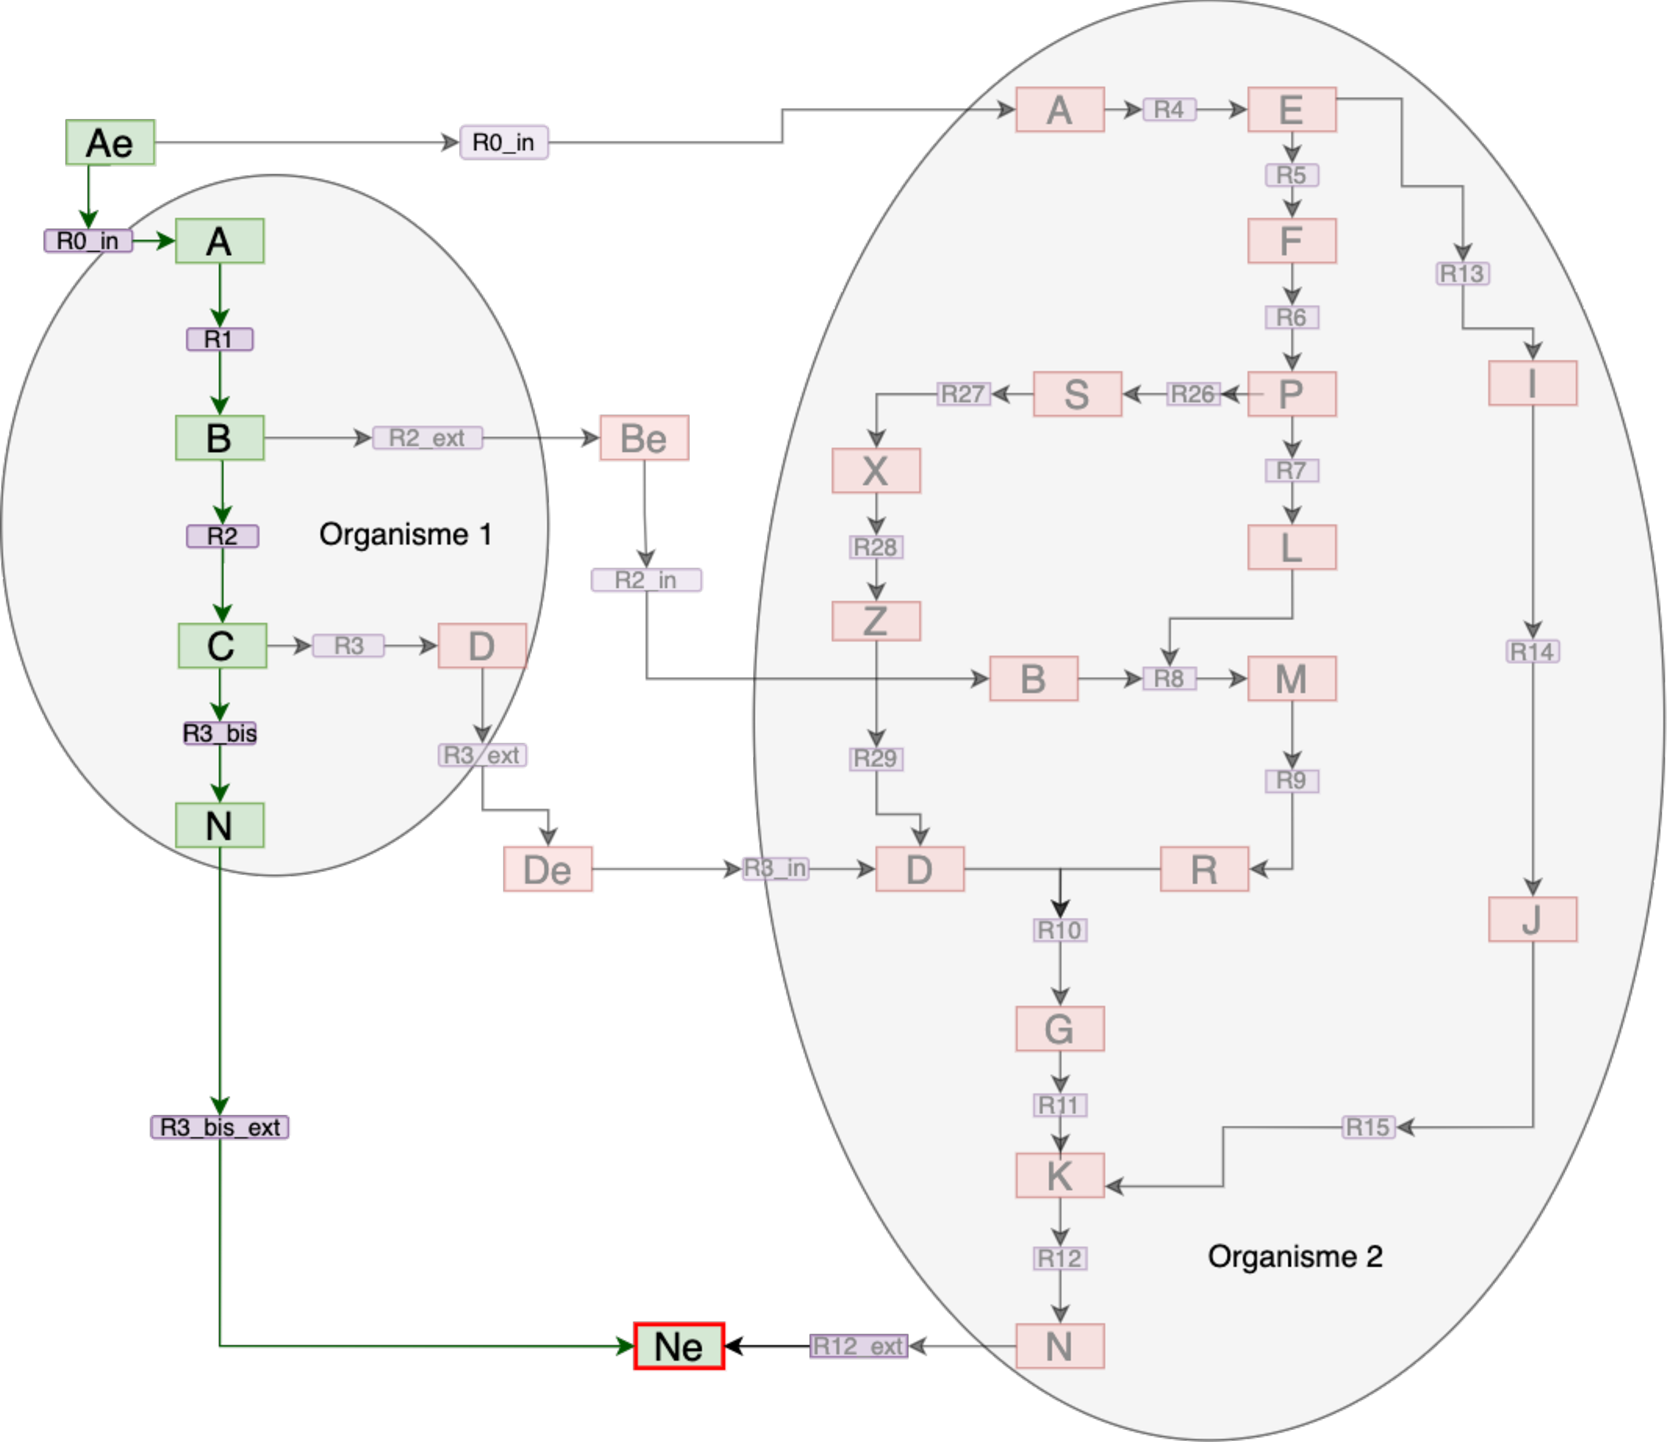
\includegraphics[scale=0.5]{img/enrichissement/Planification.pdf}
            \caption{Schéma didactique permettant de valider la solution donnée par le modèle dans le cas de la planification en montrant que le composé Ne est productible à partir d'un seul organisme via le chemin vert.}
        \label{fig:planification}
    \end{center}
\end{figure}

Aucune règle stipulant qu'une communauté est minimum composé de 2 taxons, \textit{telingo} montre que seul l'organisme 1 peut produire le composé \texttt{Ne}, comme indiqué par le listing \ref{lst:planification_res}.

\begin{lstlisting}[label =lst:planification_res, caption =Résultat de la planification obtenue après application des règles sur la base de faits, captionpos=b]
Answer: 1
 State 0:
 State 1:
  isActivated("R0_in","Org1")
  producible("A","Org1")
 State 2:
  isActivated("R1","Org1")
  producible("B","Org1")
 State 3:
  isActivated("R2","Org1")
  producible("C","Org1")
 State 4:
  isActivated("R3_bis","Org1")
  producible("N","Org1")
 State 5:
  isActivated("R3_bis_ext","Org1")
  producible("Ne","Org1")
Optimization: 1 5
OPTIMUM FOUND

Models       : 1
  Optimum    : yes
Optimization : 1 5
Calls        : 6
Time         : 0.265s (Solving: 0.00s 1st Model: 0.00s Unsat: 0.00s)
CPU Time     : 0.197s
\end{lstlisting}

Les séquences des actions montrant la production de \texttt{Ne} est représenté par “\texttt{State}" dans la sortie du modèle. Ici, Au temps réactionnel 0, aucune réaction est activée. Seul le composé extracellulaire \texttt{Ae} serait marqué comme étant \texttt{disponible}. Au temps réactionnel suivant, \texttt{State 1}, la réaction important le composé \texttt{Ae} dans le milieu intracellulaire est activé par la réaction \texttt{R0\_in} (voir ligne 4 du listing), et le composé \texttt{A} est \texttt{productible} et \texttt{disponible} (ligne 5). Au temps réactionnel suivant, \texttt{B} est \texttt{productible} et la réaction \texttt{R1} est activée. En procédant ainsi, Le composé \texttt{Ne} est \texttt{productible} et \texttt{disponible} pour l'ensemble de la communauté en 5 étapes, correspondant au temps réactionnel 5.


\subsubsection*{Vérification}
Le cas de vérification consiste simplement à vérifier qu'il existe une séquence de réactions activables permettant de produire un composé. Ainsi, nous avons vérifié la productibilité du composé \texttt{Ne}(voir listing \ref{lst:planification_res}):

Nous pouvons voir qu'à chaque pas de temps, marqué par "\texttt{State}", il existe au moins une réaction qui est activée, permettant à terme, de produire le composé \texttt{Ne}.


\subsubsection*{Explication}
Dans le cas de l'explication, nous cherchons à déterminer le chemin réactionnel permettant la production d'un composé sachant que l'on a observé la production d'un autre composé à un moment dans le temps. Brièvement, l'objectif est de savoir s’il existe une relation entre une observation faite à un moment dans le temps et l'objectif final. Dans le cas de notre exemple de l'explication représenté par la Figure \ref{fig:explication}, nous avons cherché à expliquer la production du composé \texttt{Ne} sachant que le composé \texttt{De} a été observé. Le résultat du modèle est indiqué par le tracé en vert. Le résultat du modèle est indiqué par le listing \ref{explication}:

\begin{lstlisting}[label=explication, caption=Résultat de l'explication obtenue après application des règles sur la base de faits didactique, captionpos=b]
 State 0:
 State 1:
  isActivated("R0_in","Org1") isActivated("R0_in","Org2")
  producible("A","Org1") producible("A","Org2")
 State 2:
  isActivated("R1","Org1") isActivated("R4","Org2")
  producible("B","Org1") producible("E","Org2")
 State 3:
  isActivated("R2","Org1") isActivated("R2_ext","Org1") isActivated("R5","Org2")
  producible("Be","Org1") producible("C","Org1") producible("F","Org2")
 State 4:
  isActivated("R2_in","Org2") isActivated("R3","Org1") isActivated("R6","Org2")
  producible("B","Org2") producible("D","Org1") producible("P","Org2")
 State 5:
  isActivated("R7","Org2")
  producible("L","Org2")
 State 6:
  isActivated("R3_ext","Org1") isActivated("R8","Org2")
  producible("De","Org1") producible("M","Org2")
 State 7:
  isActivated("R3_in","Org2") isActivated("R9","Org2")
  prod_explain("D","Org2")
  producible("D","Org2") producible("R","Org2")
 State 8:
  isActivated("R10","Org2")
  prod_activate("G","Org2")
  prod_activate_cof("G","Org2")
  producible("G","Org2")
 State 9:
  isActivated("R11","Org2")
  prod_activate("K","Org2")
  prod_activate_cof("K","Org2")
  producible("K","Org2")
 State 10:
  isActivated("R12","Org2")
  prod_activate("N","Org2")
  prod_activate_cof("N","Org2")
  producible("N","Org2")
Optimization: 3 17
OPTIMUM FOUND
Models       : 4
  Optimum    : yes
Optimization : 3 17
Calls        : 11
Time         : 0.366s (Solving: 0.02s 1st Model: 0.00s Unsat: 0.00s)
CPU Time     : 0.350s

\end{lstlisting}
Au temps réactionnel 6 (ligne 19), nous voyons que l'observation est expliquée, et qu'il faut attendre le temps réactionnel 10 pour que le composé final \texttt{Ne} soit productible. Nous pouvons également remarquer que le modèle explique en même temps la production du composé \texttt{Be} pour permettre la production de \texttt{Ne}: on dit alors que \texttt{Be} est un métabolite essentiel à la production de \texttt{Ne}.

\begin{figure}[H]
    \begin{center}
        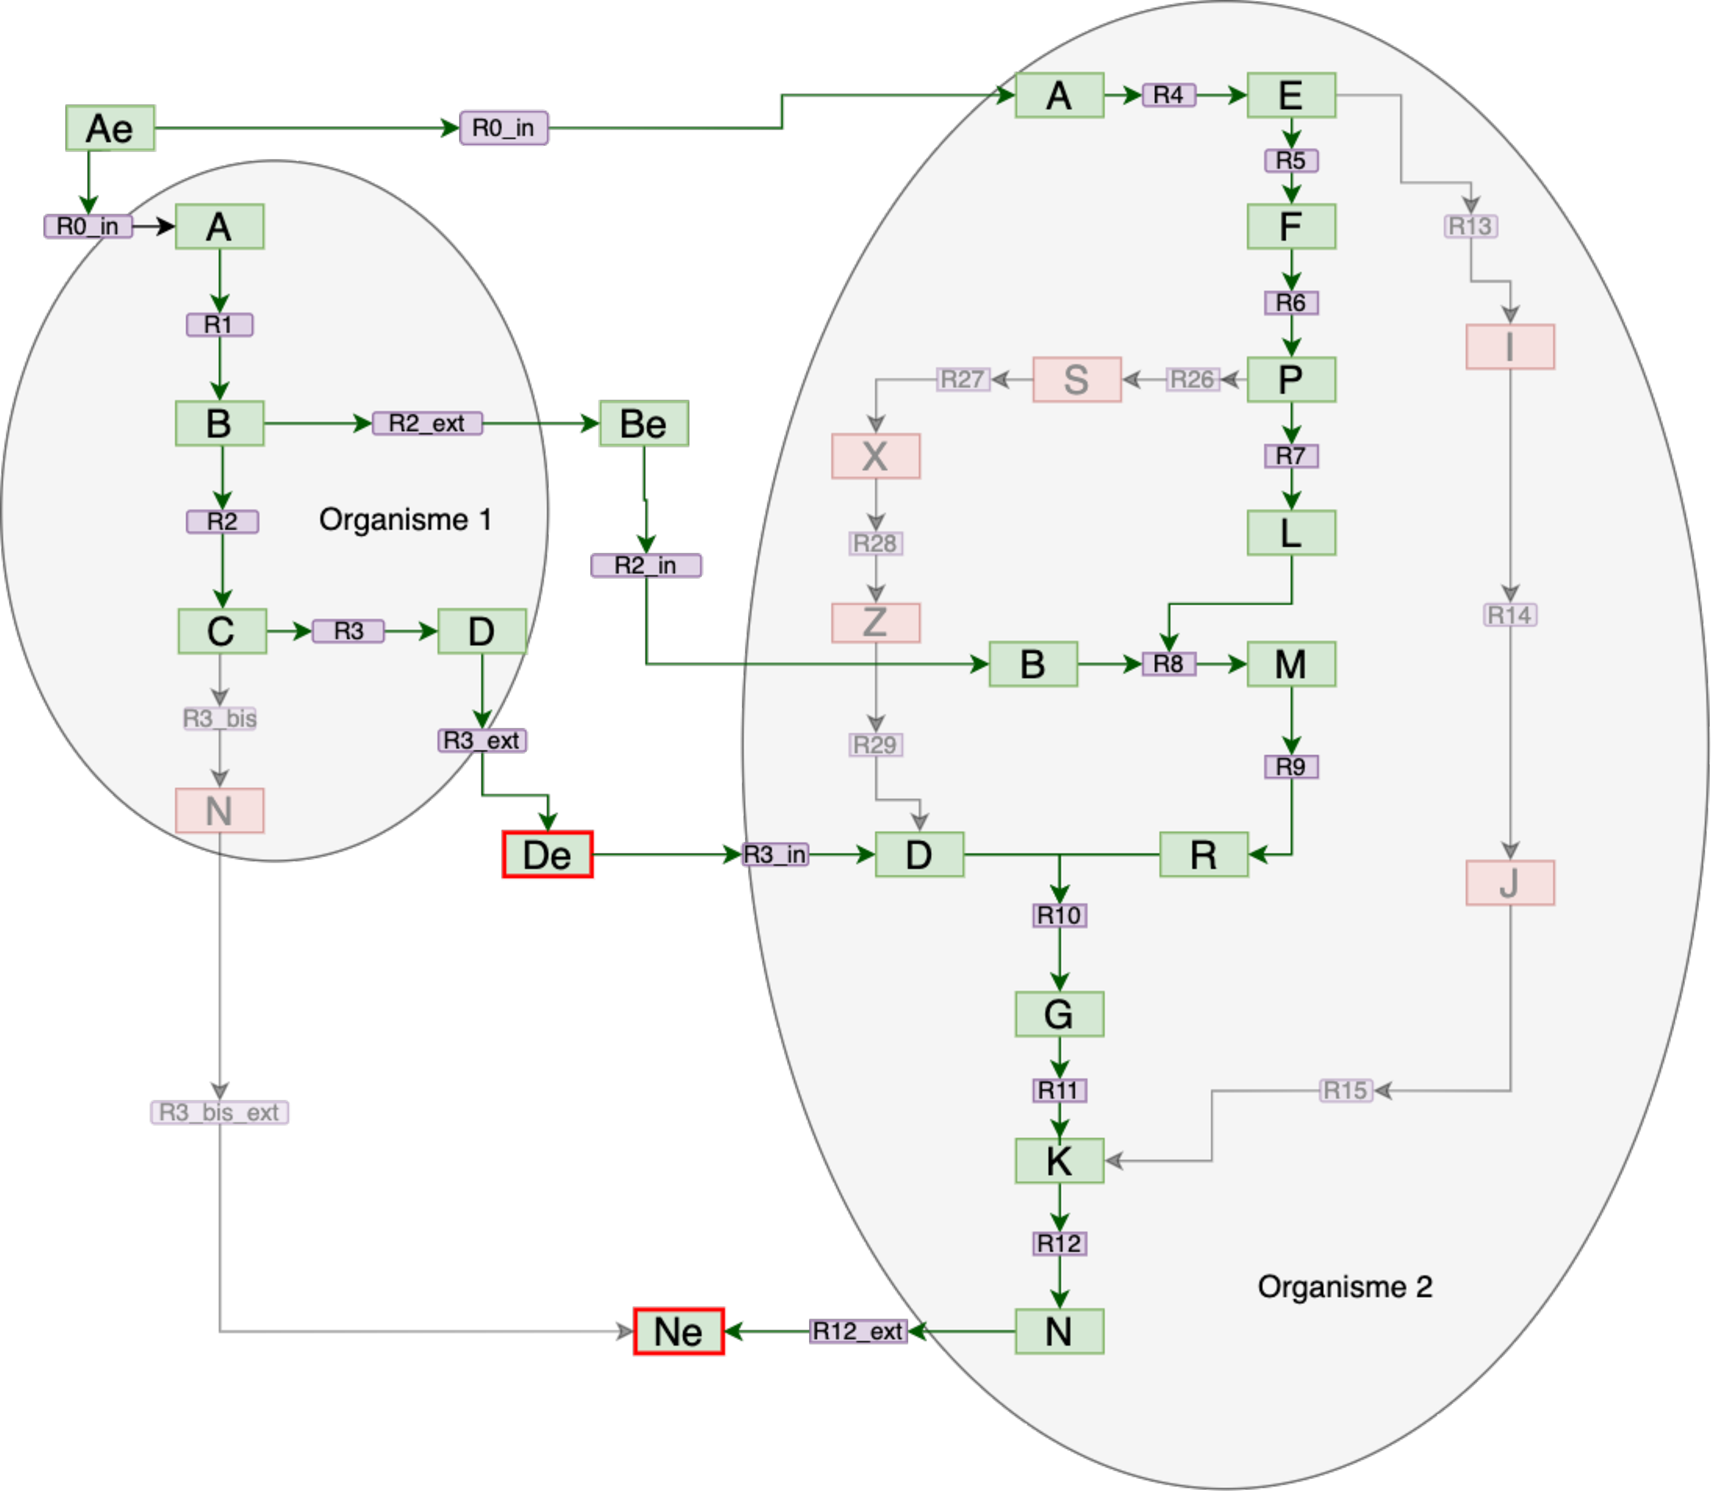
\includegraphics[scale=0.5]{img/enrichissement/Explication.pdf}
            \caption{Schéma didactique permettant de valider la solution donnée par le modèle dans le cas de l'explication en montrant que le composé Ne est productible à partir de l'élément observable De.}
        \label{fig:explication}
    \end{center}
\end{figure}
    
    
Cette implémentation temporelle, sur un schéma didactique, met en avant deux points intéressants par rapport à un dFBA. Le premier est la possibilité d'avoir la suite réactionnelle conduisant à un ou plusieurs objectifs finaux de façon direct. Cette représentation en temps réactionnel, permet donc de générer des hypothèses testables sur l'activation de ou non de voies métaboliques d'intérêt à travers des méthodes de knockout enzymatique par exemple. La seconde est la mise en avant indirect d'une coopération entre ces deux organismes. Pour rappel, la connaissance initiale montrait une observation dans le milieu extracellulaire de \texttt{De} et non un échange entre ces deux organismes. De plus, ce modèle a permis de montrer qu'un autre composé est échangé pour permettre de réaliser l'objectif final.
    
    
\section{Application à une communauté simplifié du chapitre \ref{tango}}
Nous avons repris le milieu du lait ainsi que les réseaux métaboliques du chapitre \ref{tango}, et généré la nouvelle base de faits applicable à \textit{telingo}. Nous présenterons que 2 cas: planification et explication.  \\

\subsection{Cas de la planification}
Dans le cas de la planification, le système initial est composé des 3 bactéries, du milieu nutritionnel du lait. L'objectif à attendre est la production de propionate, note \texttt{M\_ppa\_e} dans la sortie du modèle représenté par \ref{lst:planification_reel}:

\begin{lstlisting}[label = lst:planification_reel , caption = Résultat de la planification obtenue après application des règles sur la base de faits issue des données réelles]
 State 0:
 State 1:
  isActivated("R_ADK1_rev","lactis") isActivated("R_ARGDr","lactis")
  producible("M_amp_c","lactis") producible("M_atp_c","lactis") producible("M_citr__L_c","lactis") producible("M_nh4_c","lactis")
 State 2:
  isActivated("R_NTD7","lactis") isActivated("R_OCBT_rev","lactis") isActivated("R_THRD_L","lactis")
  producible("M_2obut_c","lactis") producible("M_adn_c","lactis") producible("M_cbp_c","lactis") producible("M_nh4_c","lactis") producible("M_orn_c","lactis") producible("M_pi_c","lactis")
...
...
...
 State 17:
  isActivated("R_PPAKr","lactis")
  producible("M_atp_c","lactis") producible("M_ppa_c","lactis")
 State 18:
  isActivated("R_DM_ppa_c","lactis")
  producible("M_ppa_p","lactis")
 State 19:
  isActivated("R_DM_ppa_p","lactis")
  producible("M_ppa_e","lactis")
Optimization: 1 26
OPTIMUM FOUND
Models       : 44
  Optimum    : yes
Optimization : 1 26
Calls        : 20
Time         : 65.678s (Solving: 15.03s 1st Model: 0.08s Unsat: 0.10s)
CPU Time     : 57.789s
\end{lstlisting}

Un premier résultat intéressant consiste à observer que la méthode semble passer à l'échelle d'une communauté bactérienne de taille 3 (65 secondes) composé de plusieurs milliers de réactions. Un second point surprenant concerne l'organisme qui produit le propionate: \lactis. En effet, nous savons que seul la bactérie propionique (\freud) est capable de produire ce composé. Enfin, parmi les 44 modèles, aucun ne prédit d'échanges métaboliques au sein de la communauté. \\

\subsection{Cas d'explication}
Nous avons également vu dans le chapitre \ref{tango}, que le propionate est productible à partir du lactate produit par les bactéries lactiques \lactis et \plantarum.  Ainsi, expliquer la production de propionate sachant le lactate observé et consommé par \freud constitue un exemple d'utilisation pour le cas d'explication. Nous avons représenté dans la Figure \ref{fig:explication_r}, une simplification des voies métaboliques utilisé par le modèle pour produire le propionate sachant le lactate observé.

\begin{figure}[H]
\centering
        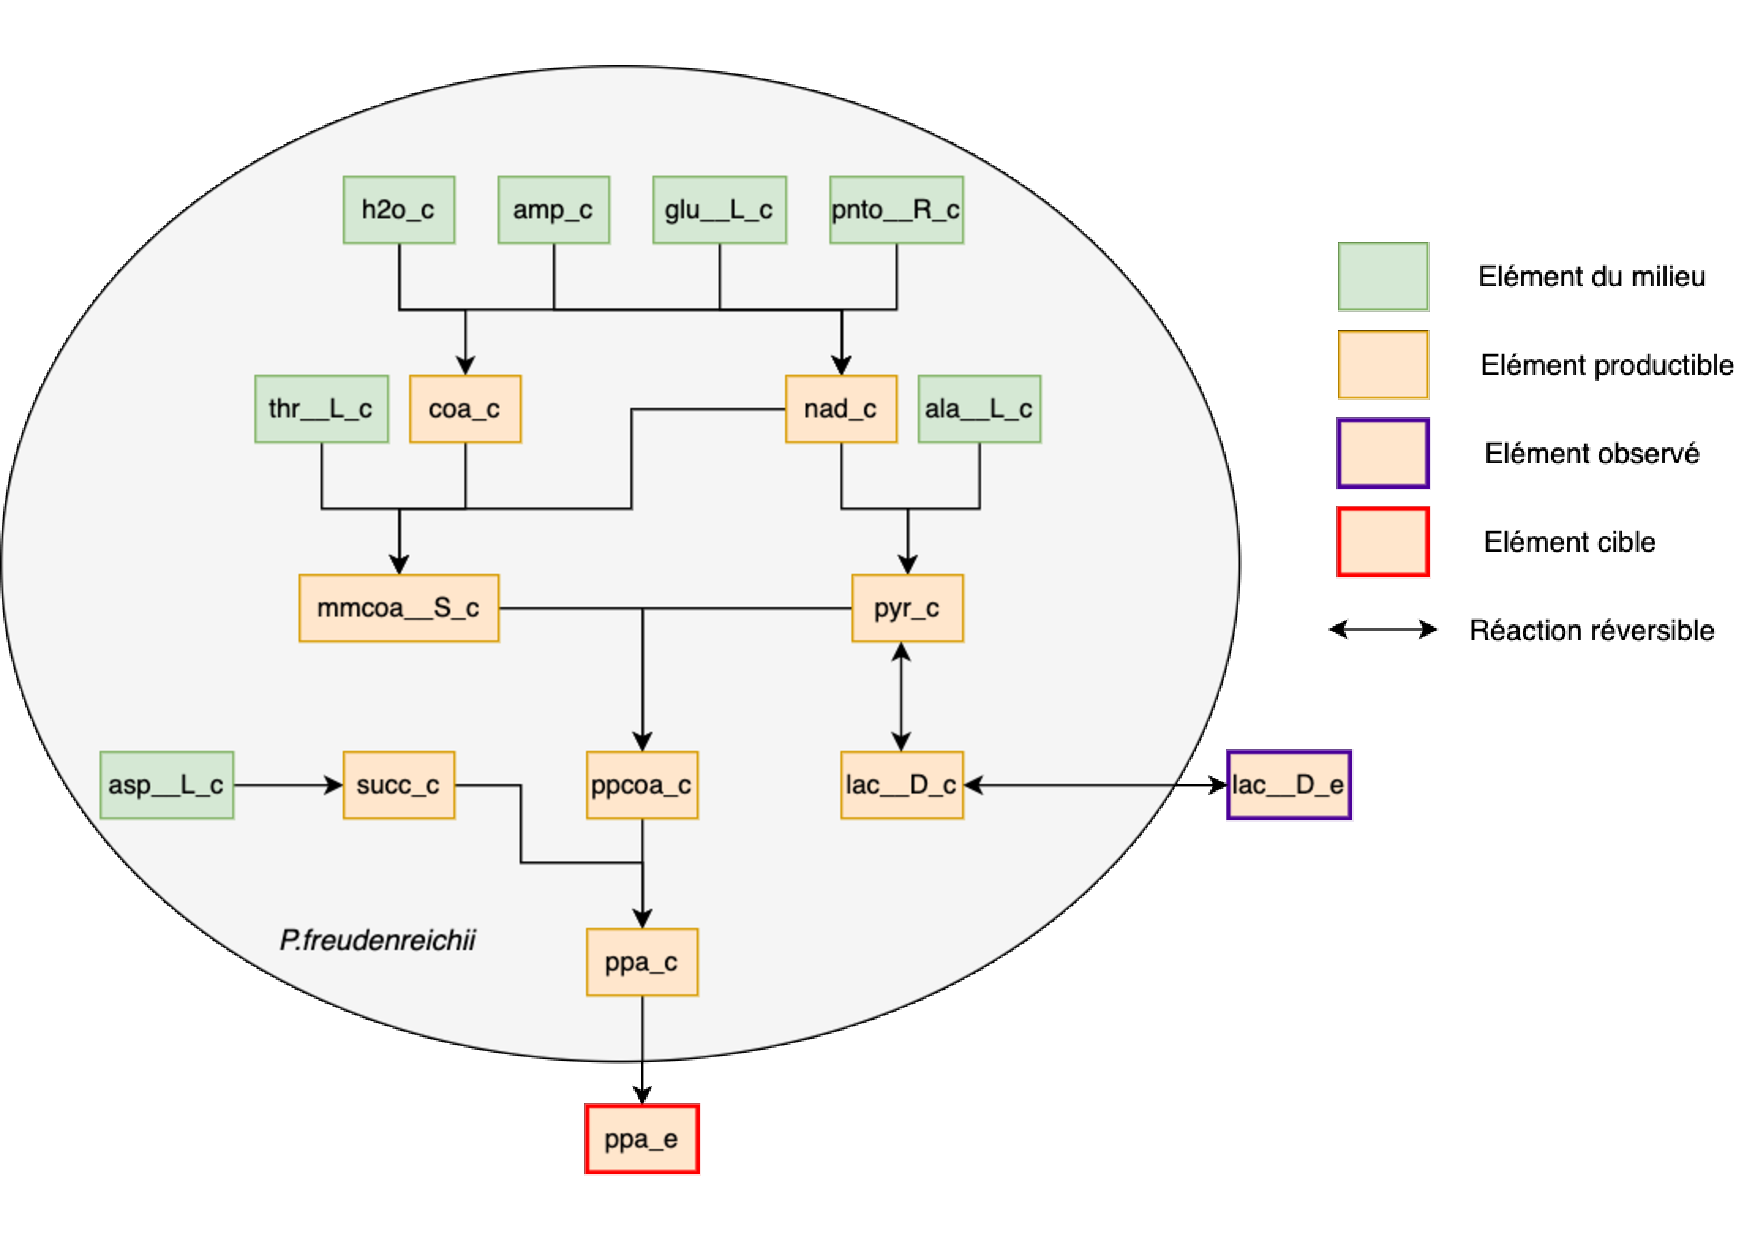
\includegraphics[width=\textwidth]{img/enrichissement/res_simplifie_v2.pdf}
            \caption{Schéma permettant de visualiser le résultat simplifié du modèle d'explication sur les données réelles}
        \label{fig:explication_r}
\end{figure}

Contrairement au cas de planification, il a fallu 23 étapes pour résoudre expliquer la production de propionate à partir du lactate. Malgré l'ajout d'une connaissance \textit{a priori} (consommation du lactate par \freud) le modèle ne permet toujours pas d'identifier les interactions entre les bactéries lactiques et la bactérie propionique. Cependant, nous pouvons reconnaître un cycle important pour la production du propionate: cycle de Wood-Werkman.


\section{Discussion et conclusion}
Nous avons montré une application à la biologie des systèmes d'un concept d'IA: le raisonnement sur les actions et le changement. Nous avons également vu l'efficacité de la temporalité sur les exemples didactiques: des hypothèses sur des interactions bactériennes , explications métaboliques d'observations et rapidité d'exécution. Tout comme dans le chapitre \ref{ccmc}, aucune fonction objective n'est nécessaire. Malgré cela, cette approche permet une description réactionnelle d'une communauté bactérienne.\\

Lors du passage à l'échelle d'un jeu de données réel, nous observons les limites d'une modélisation basée sur la topologie du réseau: production du propionate permise sans échanges métaboliques. Cependant, en sélectionnant les bonnes connaissances \textit{a priori} à inférer dans le modèle, cette modélisation topologique réactionnelle permettrait d'analyser et générer des explications rapidement sur des observations relevées lors des expériences.


\end{document}